\documentclass[a4paper]{article}
\usepackage[top = 30mm, bottom = 20mm, inner = 30mm, outer = 30mm]{geometry}

\usepackage{graphicx}
\usepackage{float}
\usepackage[english]{babel}
\usepackage[round]{natbib}
\bibliographystyle{abbrvnat}
\bibliographystyle{plainnat}
\usepackage{subcaption}

\usepackage[hidelinks]{hyperref}

\usepackage{booktabs}	% lässt \top-, \mid- & \bottomrule in Tab zu

\usepackage{multicol}

\usepackage{titlesec}
\titleformat{\section}
{\normalfont\fontsize{11}{13}\bfseries}{\thesection}{1em}{}

\renewcommand{\figurename}{Fig.}
\renewcommand{\thefigure}{S\arabic{figure}}
\renewcommand{\tablename}{Tab.}
\renewcommand{\thetable}{S\arabic{table}}

\renewcommand*{\contentsname}{Table of Contents}

\usepackage{todonotes}

\usepackage{xr}
\externaldocument{OnOffRivers_0_Paper}
\externaldocument{OnOffRivers_OSM_1_SupplFigures}
\externaldocument{OnOffRivers_OSM_3_Petrography}


%opening
\title{Online Supplemental Material (OSM) 2: Description of sampled sites}
%\author{Dirk Seidensticker}

\begin{document}

\setcounter{figure}{6}
\setcounter{table}{1}

\maketitle

\tableofcontents

\vspace{20em}

\section{Pikunda on the middle Sangha river}

The site of Pikunda on the Sangha river (Fig.~\ref{fig:map}) was discovered in 1987 during fieldwork of the \textit{River Reconnaissance Project}, led by Manfred K. H. \citet{Eggert.1992,Eggert.1993}. Subsequent to foot-surveys, which yielded 279 sherds \citep[345]{Seidensticker.2021e}, three locations for small-scale excavations were determined \citep[288--305]{Seidensticker.2021e}. Trench 1 (PIK~87/1) yielded a 3.4~m deep pit that contained mostly ceramics of the Pikunda-Munda style dating into the 2nd century BCE to 5th century CE \citep[Fig.\ref{fig:chrono};][114--120]{Seidensticker.2021e}. This feature was cut by another, 0.9~m deep pit that contained mostly pottery of the Mandombe style dating into the 14th to 15th century CE \citep[Fig.\ref{fig:chrono};][145--148, 291 Fig.~133, 293 Fig.~135B]{Seidensticker.2021e}. A nearby, 1.5~m deep pit (PIK~87/2) dated into the second half of the 20th century CE \citep[300--301]{Seidensticker.2021e}. The third feature excavated at Pikunda (PIK~87/3) is a shallow slag-tapping open-bowl furnace that dates into the 11th to 13th century CE \citep[299 Fig.~138, 301--305]{Seidensticker.2021e}. The infill of the connected slag pit contained pottery associated with the Ebambe style \citep[131--136]{Seidensticker.2021e}. In addition to the excavations, ethnographic observations also documented the potting of multiple ceramic vessels by a local potter \citep{Eggert.inVorb.}.

\begin{figure}[p]
	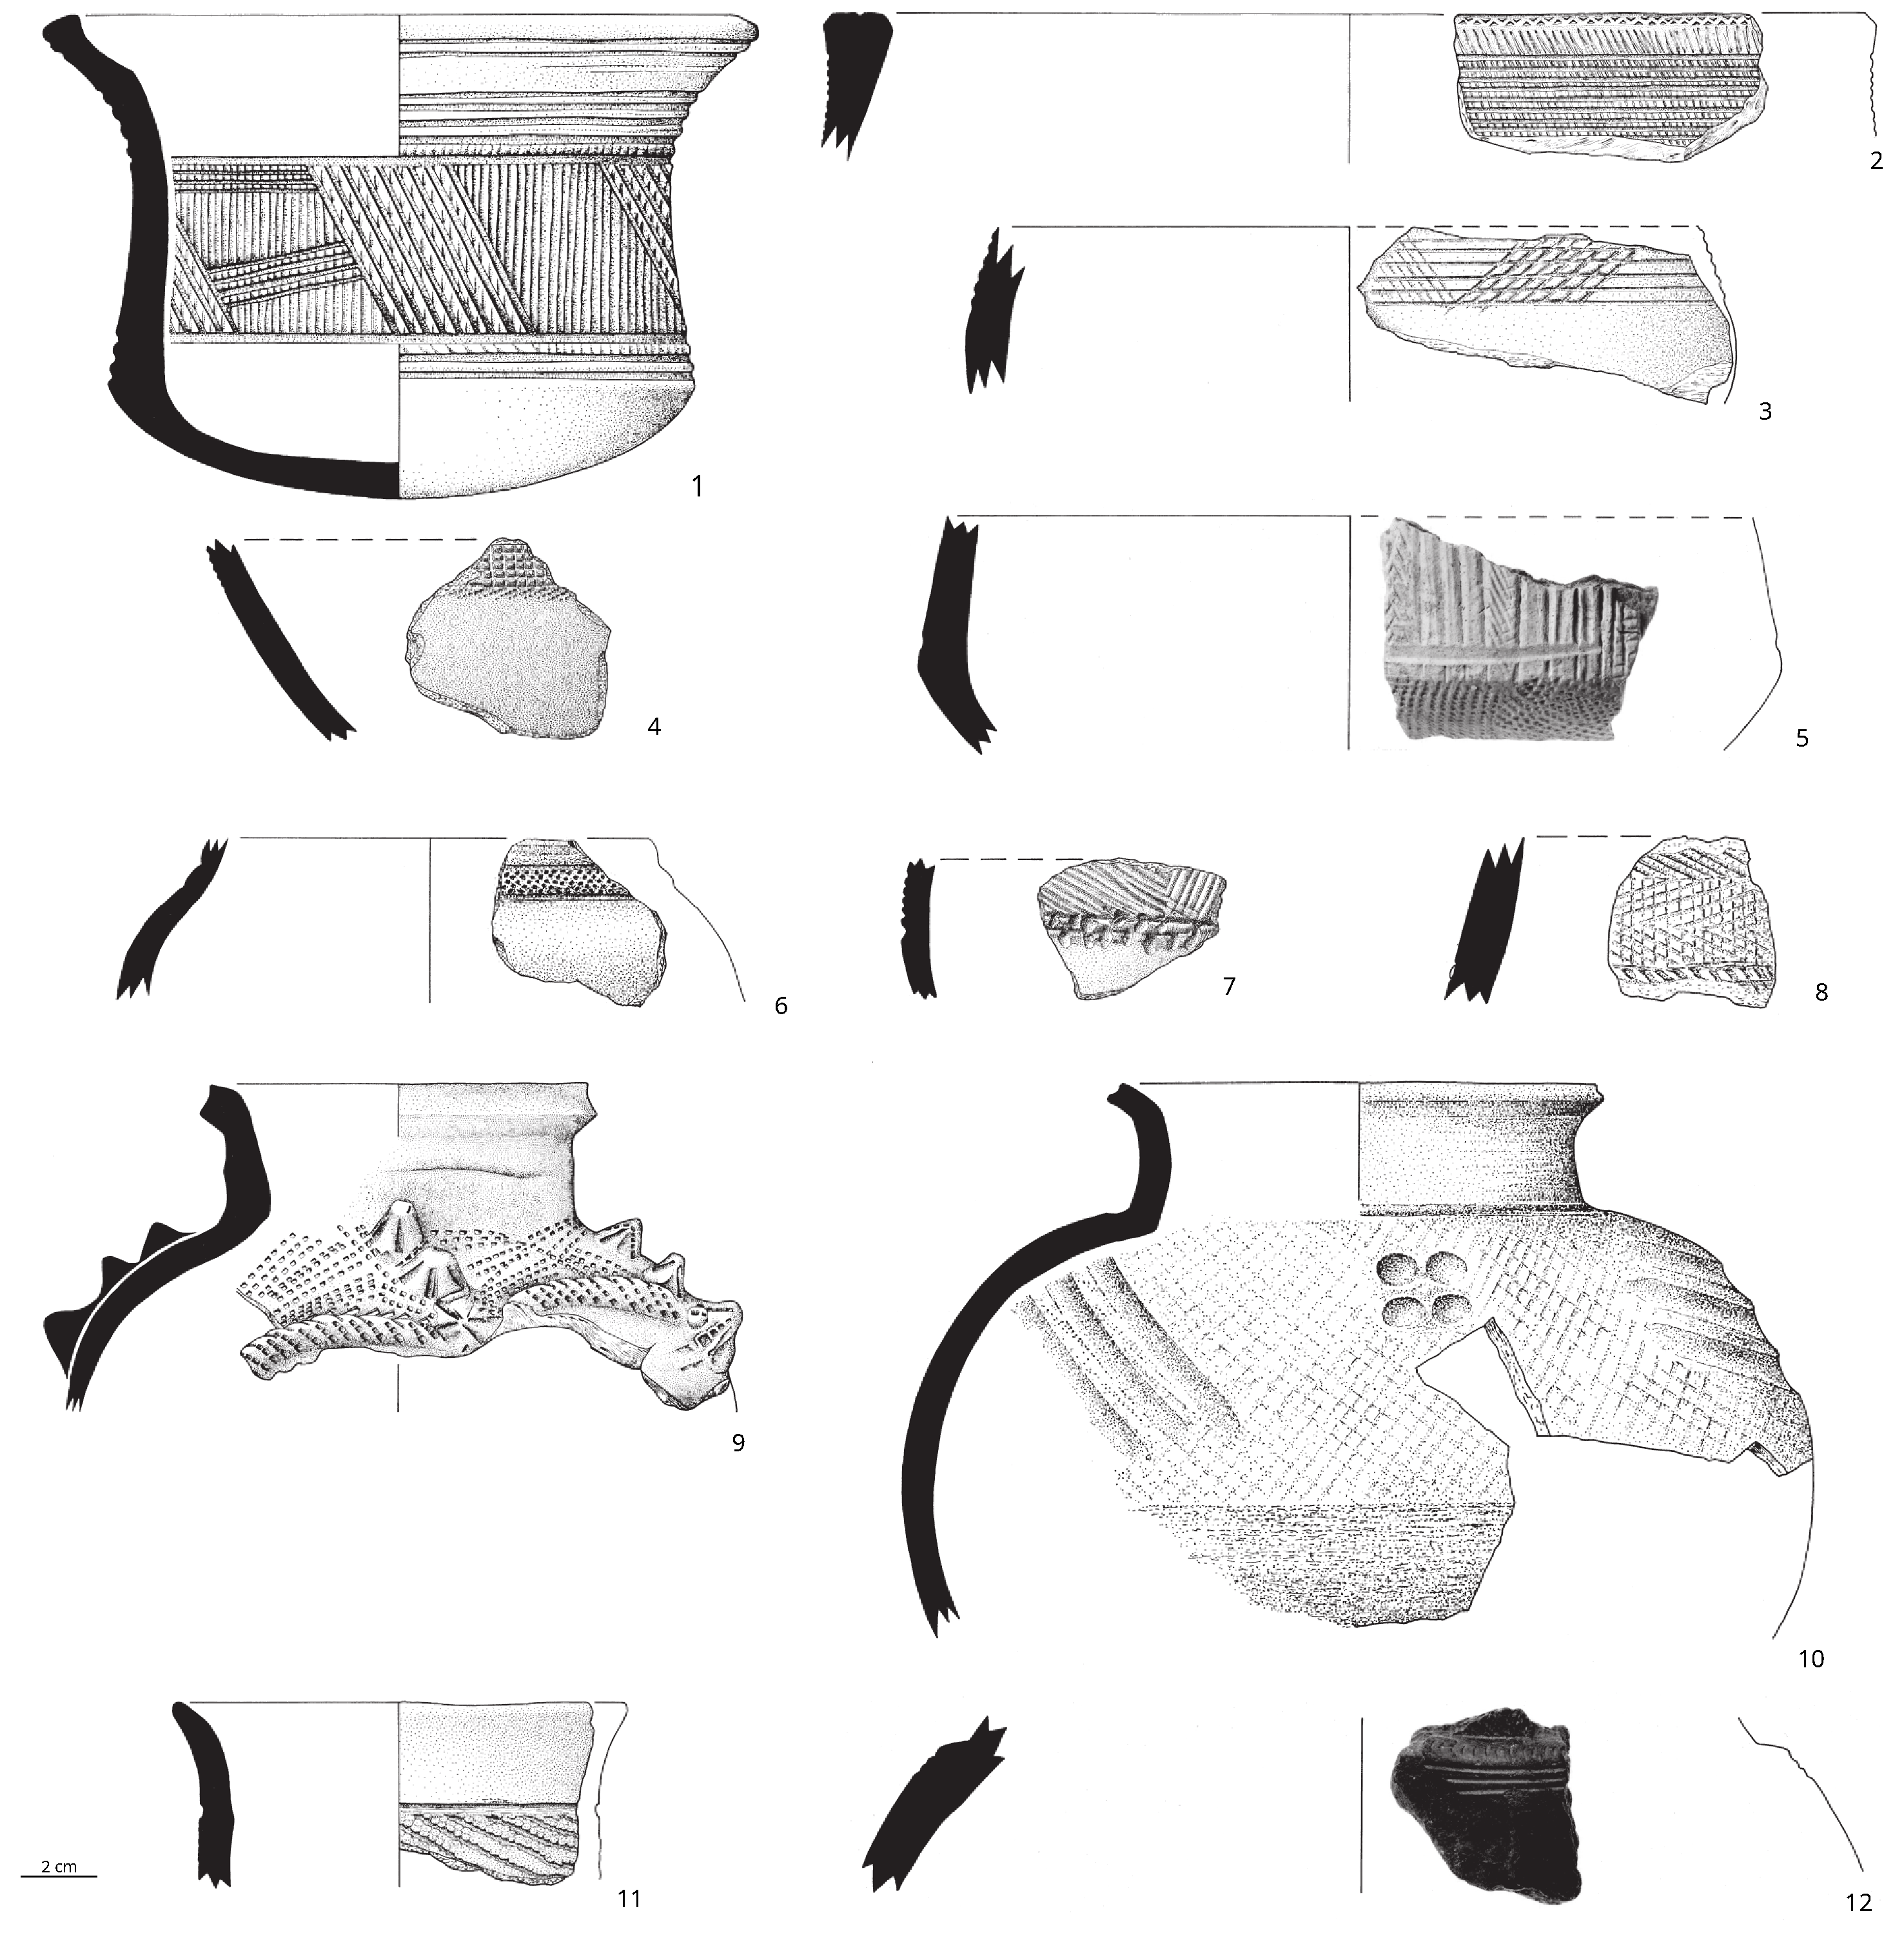
\includegraphics[width=\textwidth]{Fig_Pikunda_PotterySampled.pdf}
	% Pikunda-Munda style
	% 2: PIK 87/1-12:1 (45.16)
	% 3: PIK 87/1-5:1 -6:10 -7:12 -9:6 (46.21)
	% 4: PIK 87/1-9:5 (47.6)
	% 5: PIK 87/2-4:73 (48.25)
	% Ngbanja style
	% 6: PIK 87/1-8:1 (47.20)
	% 7: PIK 87/1-8:2 (47.21)
	% 8: PIK 87/1-9:7 (47.19)
	% modern
	% 11: PIK 87/2-6:52 (49.5)
	% Ebambe style
	% 12: PIK 87/2-1:40 (49.10)
	\caption{Pottery from Pikunda representing the pottery styles Pikunda-Munda (1, 3--5), Lusako (2), \textit{cf}. Ngbanja (6--8), Mandombe (9--10), and Ebambe (12).}
	\label{fig:pik.pottery}
\end{figure}

\begin{figure}[p]
	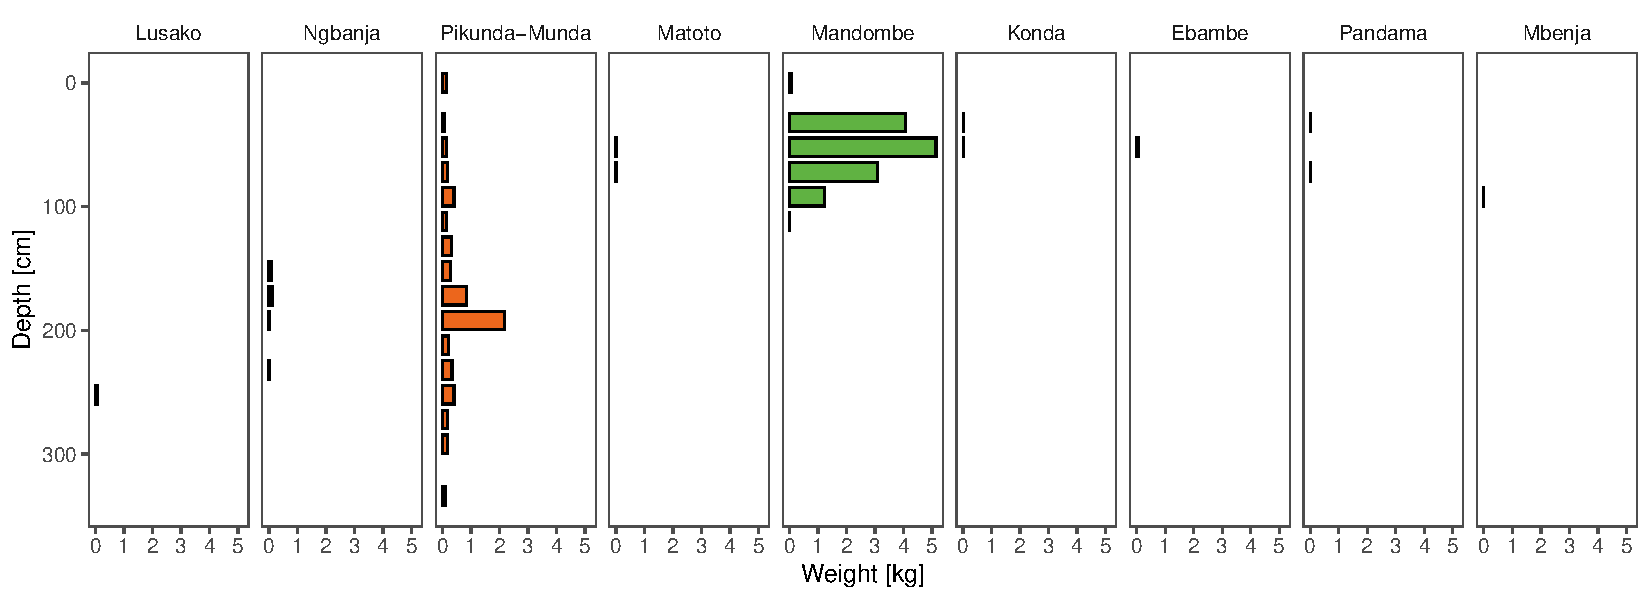
\includegraphics[width=\textwidth]{Fig_PIK87-1_Po_Wgt.pdf}
	\caption{Vertical distribution of pottery found in the excavation of trench PIK~87/1 in Pikunda \citep[cf.][293 Fig.~135.D]{Seidensticker.2021e}. Colors are corresponding to Fig.~\ref{fig:chrono}.}
	\label{fig:pik87_1.pottery}
\end{figure}

\begin{figure}[H]
	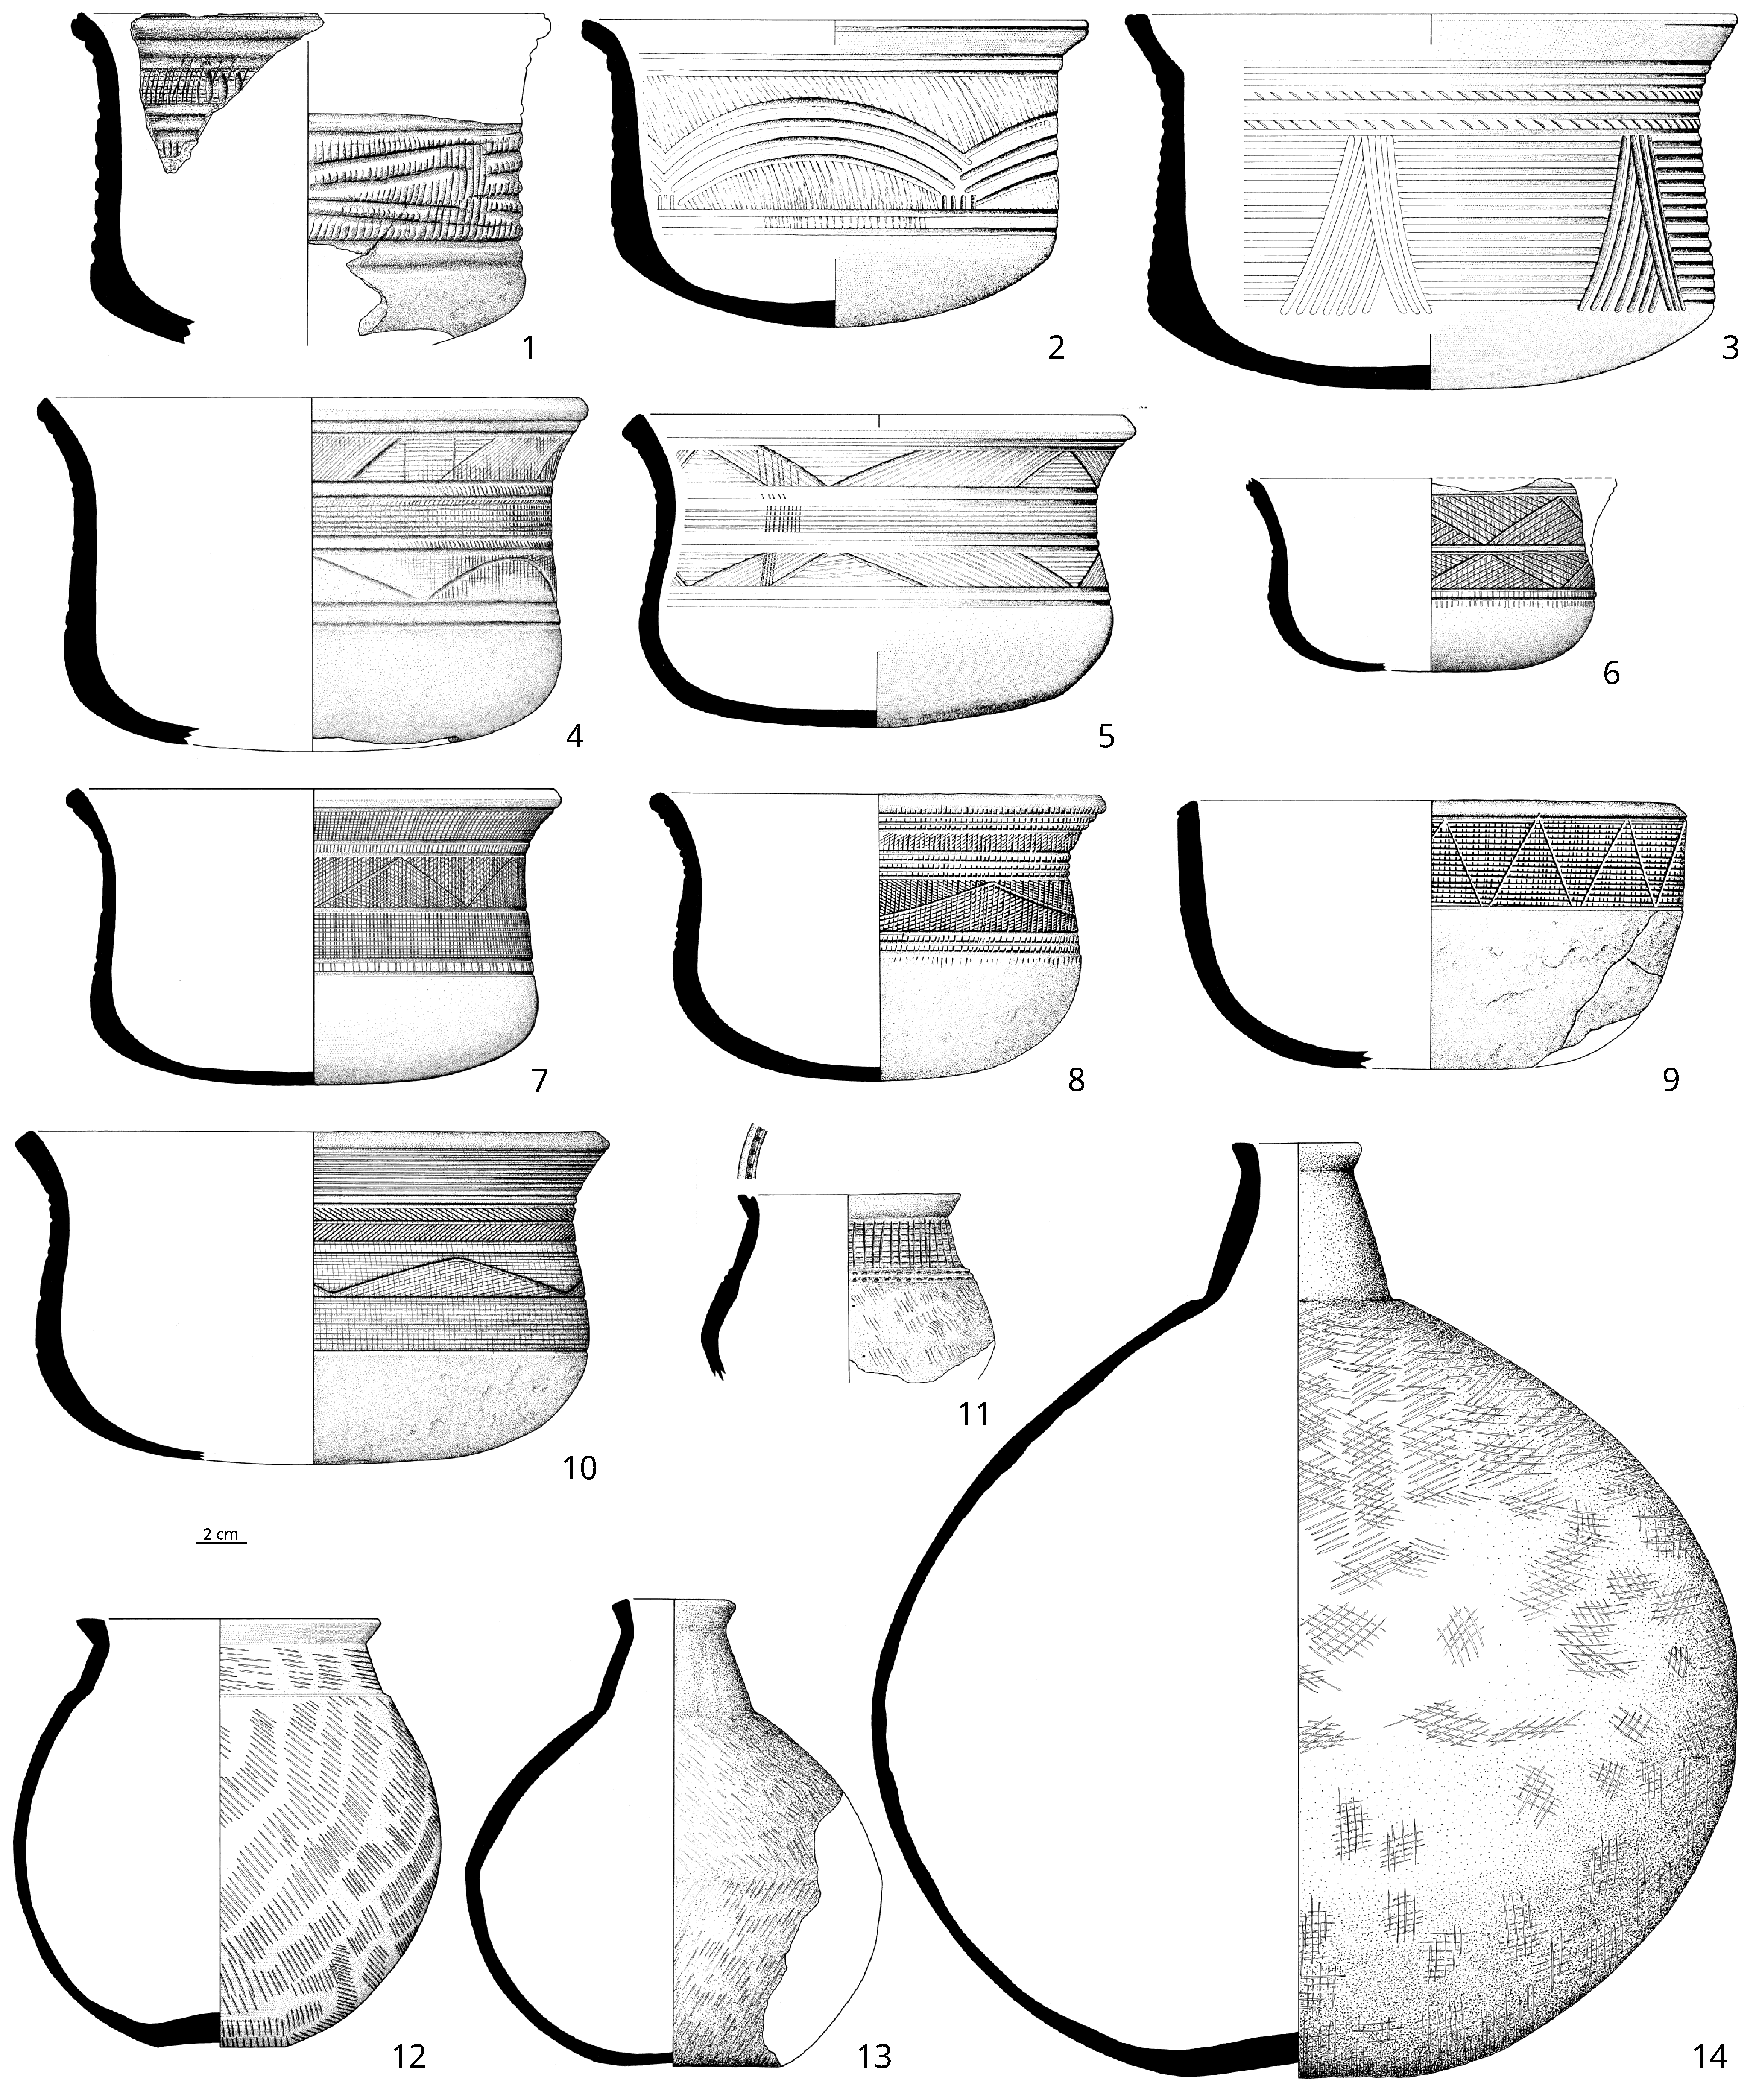
\includegraphics[width=\textwidth]{Fig_Munda_PotterySampled.pdf}
	% Pikunda-Munda style
	% 1: MUN 87/2-1-1-2:2 (91.2)	
	% 2: MUN 87/2-1-1-4:2 (91.1)
	% 3: MUN 87/2-1-1-5:2 (91.5)
	% 4: MUN 87/2-1-1-8:3 (91.7)
	% 5: MUN 87/2-1-1-8:1 (91.8)
	% 6: MUN 87/2-1-1-7:2 (91.6)
	% 7: MUN 87/2-1-3-1:2 (92.2)
	% 8: MUN 87/2-1-3-4:4 (92.4)
	% 9: MUN 87/2-1-3:3 (92.5)
	% 10: MUN 87/2-1-3:7 (93.1)
	% Ebambe style
	% 11: MUN 87/1-0-2-4:2 (89.2)
	% 12: MUN 87/1-0-2-1:1 (89.4)
	% 13: MUN 87/1-0-2-6:2 (90.1)
	% 14: MUN 87/1-0-2-6:1 (90.2)
	\caption{Pottery from Munda representing the pottery styles Pikunda-Munda (1--10) and Ebambe (11-14).}
	\label{fig:mun.pottery}
\end{figure}

\section{Munda on the upper Likwala-aux-Herbes river}

Munda on the upper Likwala-aux-Herbes river (Fig.~\ref{fig:map}) was surveyed during the 1987 fieldwork of the \textit{River Reconnaissance Project} \citep{Eggert.1992,Eggert.1993}. During foot-surveys that yielded 43 sherds \citep[349]{Seidensticker.2021e}, a yard with multiple discolorations and concentrations of pottery visible at the surface was discovered. Subsequently four small-scale excavations were conducted.

In the first trench (MUN 87/1) two features were excavated. A shallow pit with a diameter of about 0.6~m, reached to about 0.4~m below the surface \citep[311--321]{Seidensticker.2021e}. The infill consisted manly of iron slag and the upper 20~cm of the infill showed a angular fired lining along the pits western, northern and north-eastern walls \citep[315 Fig. 151--152]{Seidensticker.2021e}. The adjacent pit, which was around 1.4~m in diameter and reached up to 0.7~m below the ground, yielded a rich inventory of complete or partially complete ceramic vessels (Fig.\ref{fig:mun.pottery}.11--14), many deposited lying on their sides, and dating younger than the 16th century CE (\citeauthor{Seidensticker.2021e}, \citeyear{Seidensticker.2021e}, 320 Tab.~45; \citeauthor{Seidensticker.2024}, \citeyear{Seidensticker.2024}, Tab.~2). 

About eight meters to the north-west, two dark discolorations of the soil and ceramic fragments on the surface were observed and subsequently excavated. The trench (MUN~87/2) yielded two adjacent pit features, each about 1.4--1.5~m deep and 0.9--1.1~m in diameter \citep[321--335]{Seidensticker.2021e}. The southern of the two pits (MUN~87/2-1-1) displayed a distinct sequence of usages \citep[329 Fig.~163]{Seidensticker.2021e}: the initial, 1.5~m deep pit, was filled at least partially with sediment and four bowls \citep[473 Pl.~91.6--8]{Seidensticker.2021e} that were deposited lying on their sides \citep[323 Fig.157G--H]{Seidensticker.2021e}. After that, the upper part of the pit, up to around 0.9~m below the modern surface, was fitted with a clay lining and presumably used for metallurgical purposes, as the lining turned fire-hardened. Afterwards the feature must have been emptied and a second deposition, consisting of seven bowls \citep[473 Pl.~91.1--5]{Seidensticker.2021e} as well as at least 7.5~kg of slag was placed in the upper part of the feature. The bowls deposited in the upper infill were also placed lying on their sides or mouths \citep[323 Fig.157A--E]{Seidensticker.2021e}. It is impossible to retrace the temporal distance between the first deposition, the metallurgical processes and the second deposition due to the very high standard errors of the conventional radiocarbon dates. Two samples from each infill were analyzed, but after calibration all four dates overlap \citep[328 Fig.~162]{Seidensticker.2021e}. While the two samples from the lower infill (Tab.~\ref{tbl:c14_pik}: KI-2881 \& KI-2886) showed a consistent, overlapping age range, the samples from the upper part (Tab.~\ref{tbl:c14_pik}: KI-2885 \& KI-2887) span nearly a whole millennia after calibration. Noteworthy is a slight stylistic difference between the bowls deposited in the two distinct infills: while all bowls belong to the diagnostic type of the Pikunda-Munda style, wide, open-mouthed bowls with approximately parallel or concave sides, flared rims and round bases, the bowls from the lower part show a rounded transition from the wall to the base (Fig.~\ref{fig:mun.pottery}.4--6), while the bowls from the upper infill all show a distinctly carinated profile (Fig.~\ref{fig:mun.pottery}.1--3). 

The neighboring pit (MUN~87/2-1-3) showed a comparatively less complex usage history. A 1.4~m deep pit with a diameter of around 0.8~m was backfilled with a collection of at least 21 vessels, all pertaining to the Pikunda-Munda style \cite[Fig.\ref{fig:mun.pottery}.7--10;][114--120; 330--335]{Seidensticker.2021e}. These vessels are not evenly distributed in the infill, but were deposited either lying on sides or mouths in three distinct concentrations: five bowls were placed near the base of the pit, seven bowls were deposited around a single bigger vessel between 0.5--0.8~m below the modern surface, and eight vessels were deposited in the upper part of the feature \cite[331 Fig.~164]{Seidensticker.2021e}. The two radiocarbon dates obtained from this pit (Tab.~\ref{tbl:c14_pik}: KI-2876 \& KI-2888) place it into the same time-span as the neighboring pit MUN~87/2-1-1.

\begin{figure*}[!tb]
	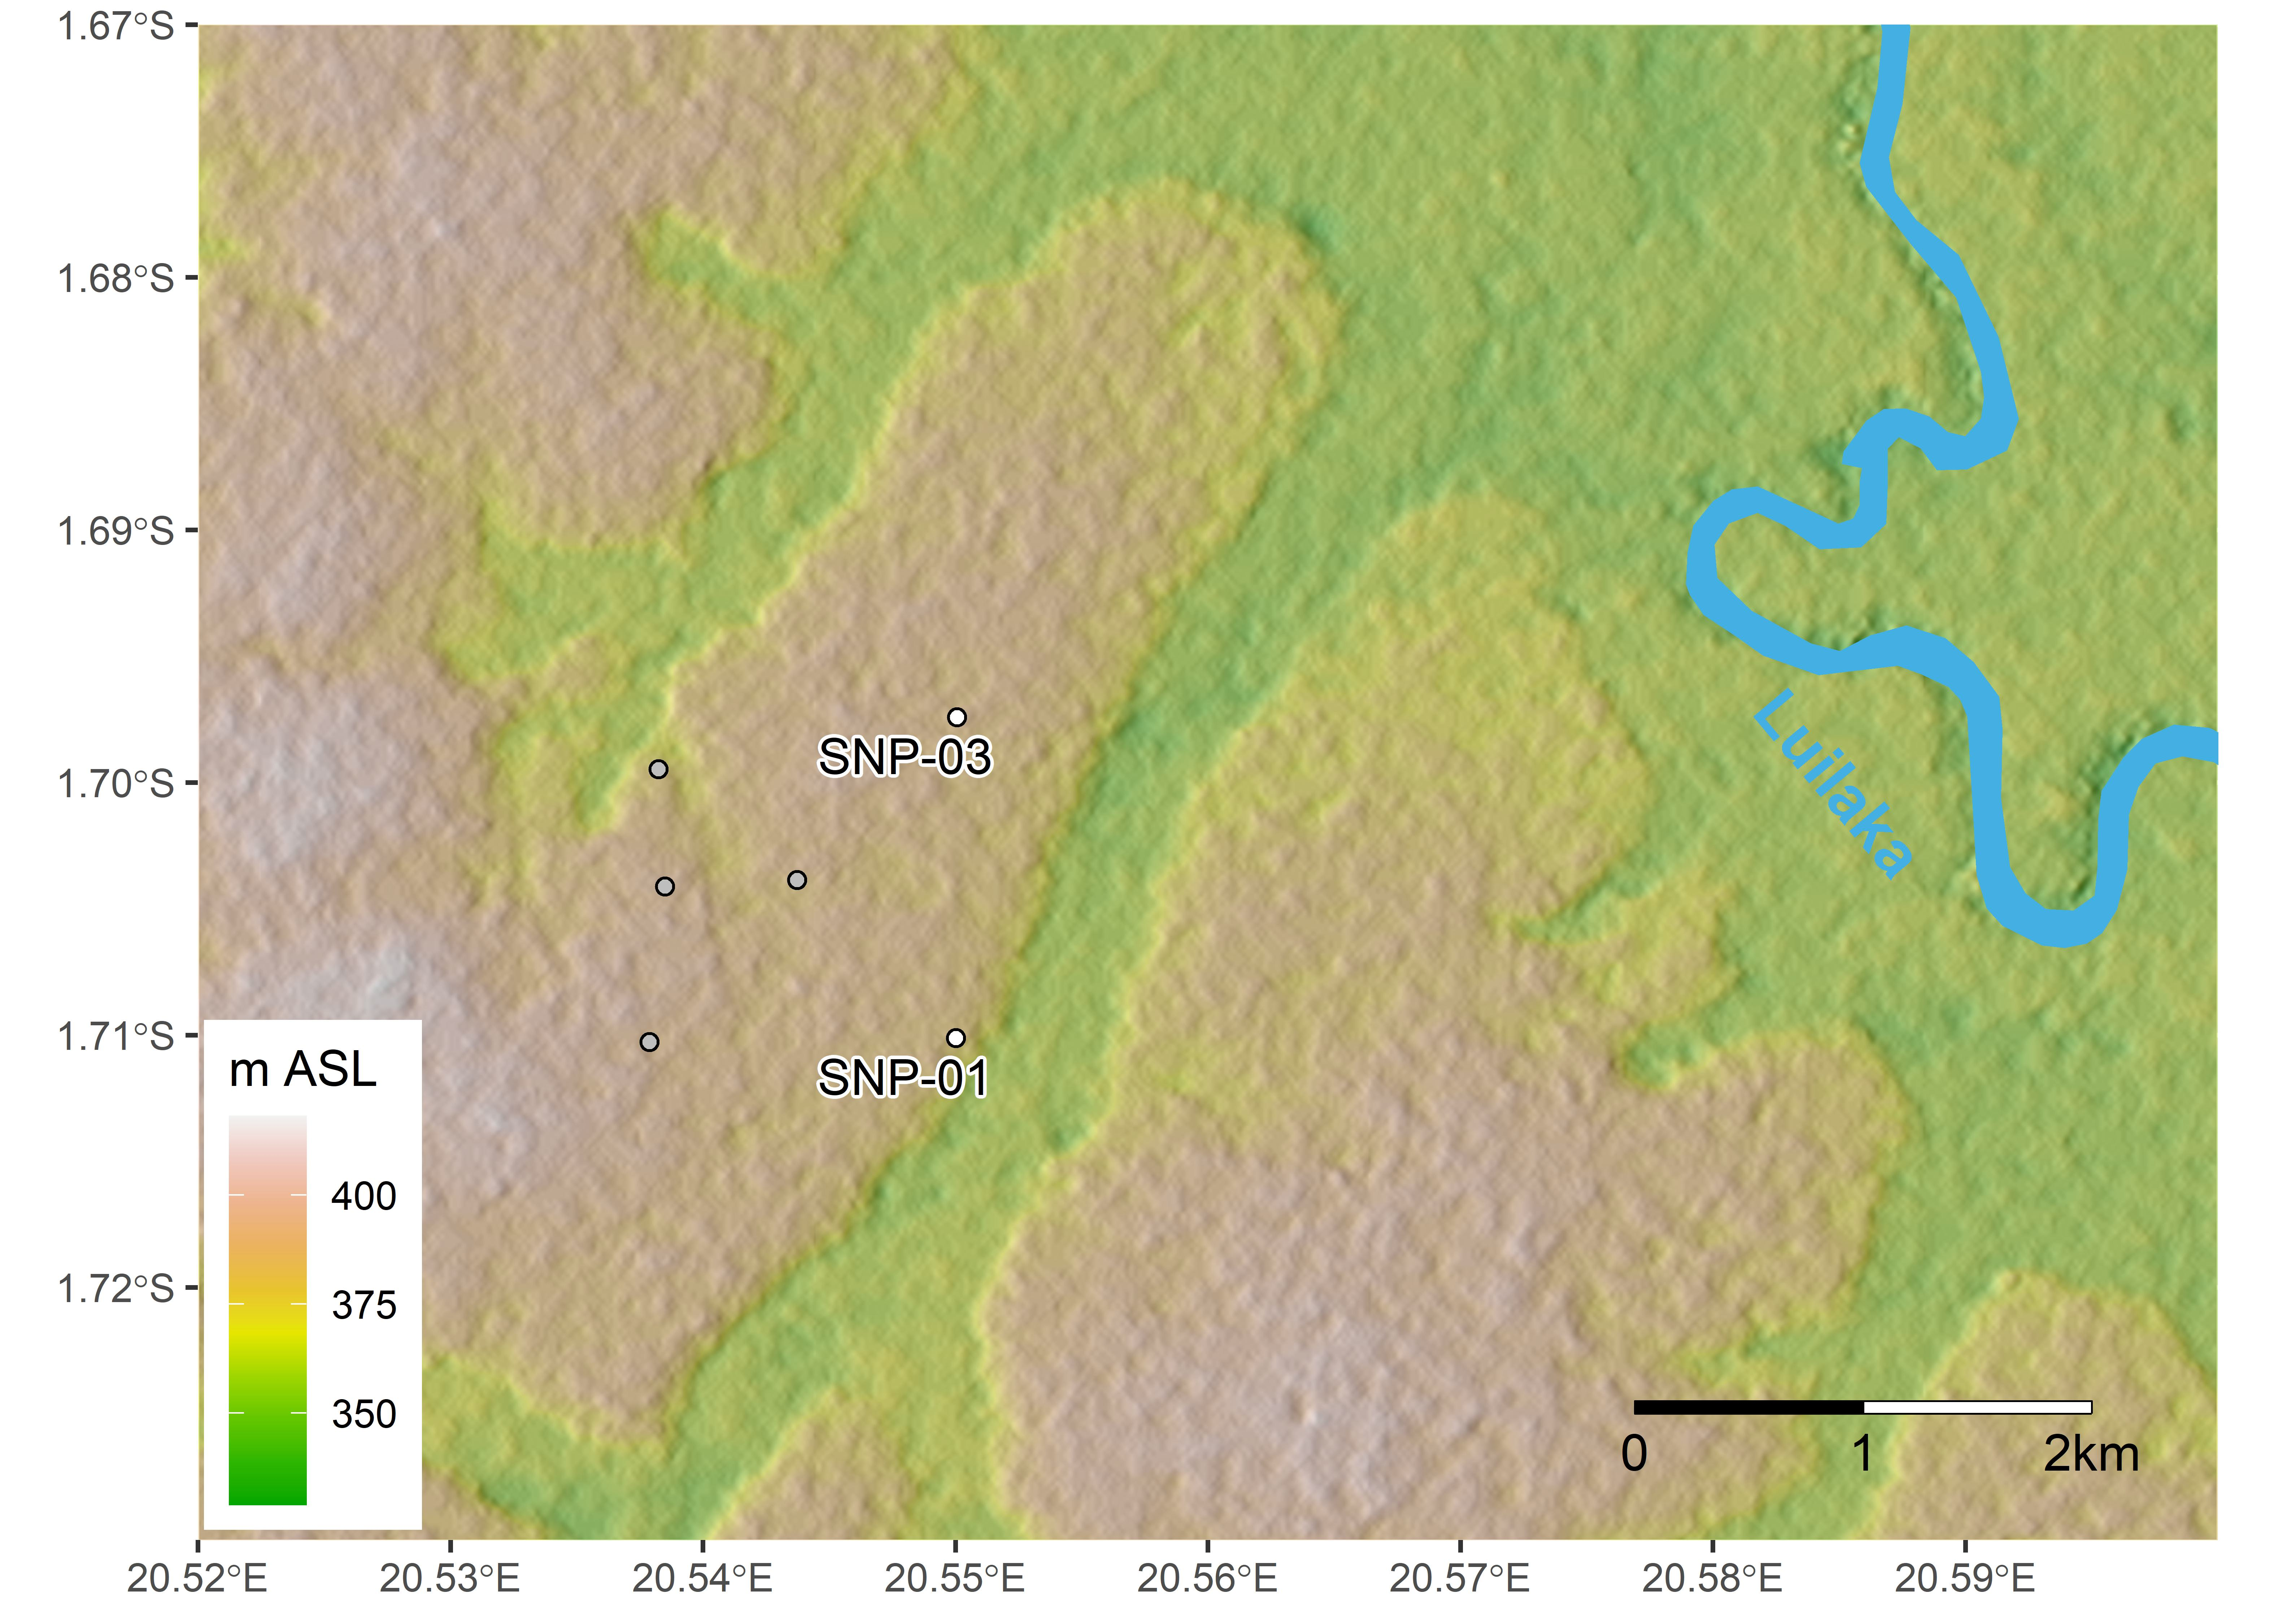
\includegraphics[width=\textwidth]{Fig_Terrain_SNP.jpg}
	\caption{Topographic map of the sampling locations SNP-01 \& SNP-03.}
	\label{fig:snp.map}
\end{figure*}

\section{Pedo-anthracological trenches in the Salonga national park (Luilaka river)}

Two out of five pedo-anthra\-cological test pits in the Salonga National Park (SNP-01 \& SNP-03) yielded fragments of ceramic vessels. Both pits are about 3.2--3.7~km east of the Luilaka river and about 1.4~km apart from each other on the 'terra firme' (Fig.~\ref{fig:map}B; \ref{fig:snp.map}). Pit SPN-01 is located at the southern edge of a small plateau, about 28 meters above the Luilaka river, while SNP-03 is situated a bit higher on the same plateau and around 52 meters above the level of the Luilaka (Fig.~\ref{fig:snp.map}). In total 640~g of ceramic material were discovered (Tab.~\ref{tab:snp.pottery}). Pit SNP-01 only yielded eight sherds, pertaining to the same vessel unit, found between 60--70~cm below the surface (Fig.~\ref{fig:snp.pottery}.1). This spit was dated into the 4th century BCE to 1st century CE (Fig.~\ref{fig:c14}; Tab.~\ref{tbl:c14_slg}: RICH-25306), while an upper spit between 30--40~cm dates into the late 15th to early 17th century CE (Fig.~\ref{fig:c14}; Tab.~\ref{tbl:c14_slg}: RICH-25315). 55 sherds were found in the upper 70~cm in pit SNP-03, while the bulk of material was found between 30--40~cm below the surface (Tab.~\ref{tab:snp.pottery}). This spit was radiocarbon dated between the late 8th to 10th century CE (Fig.~\ref{fig:c14}; Tab.~\ref{tbl:c14_slg}: RICH-25317). The pottery found in SNP-03 is heavily fragmented, with 71~\% being smaller than 3~cm and 27~\% of sherds being 3--7~cm in size. The bulk of sherds are undecorated wall fragments (91~\%). Of special importance are ten sherds that are part of an ovaloid pot with short everted rim and slightly conical shoulder area \citep[Fig.~\ref{fig:snp.pottery}.5; \textit{cf}. type B4][30 Fig.~5]{Seidensticker.2021e}. Four sherds are fragments of vessels with short, concave, everted rims (Fig.~\ref{fig:snp.pottery}.2,3,7). Only three sherds showed any remnants of decoration: a very small sherds shows impressions with a comb (Fig.~\ref{fig:snp.pottery}.6), a second sherd shows a groove and round impressions (Fig.~\ref{fig:snp.pottery}.4), and the third sherd shows a groove right underneath the rim (Fig.~\ref{fig:snp.pottery}.7). The single vessel unit obtained from SNP-01, consisting of eight sherds, was clearly made out of fluvial clays rich in sponge spicules (Fig.~\ref{fig:43_snp}). Its shape is reminiscent of the flat bases with a single groove that is characteristic for the Bokuma pottery style \citep[Fig.~\ref{fig:snp.pottery}.1; \textit{cf}. type B10][117, 440 Pl.~6]{Wotzka.1995}.

\begin{figure*}[p]
	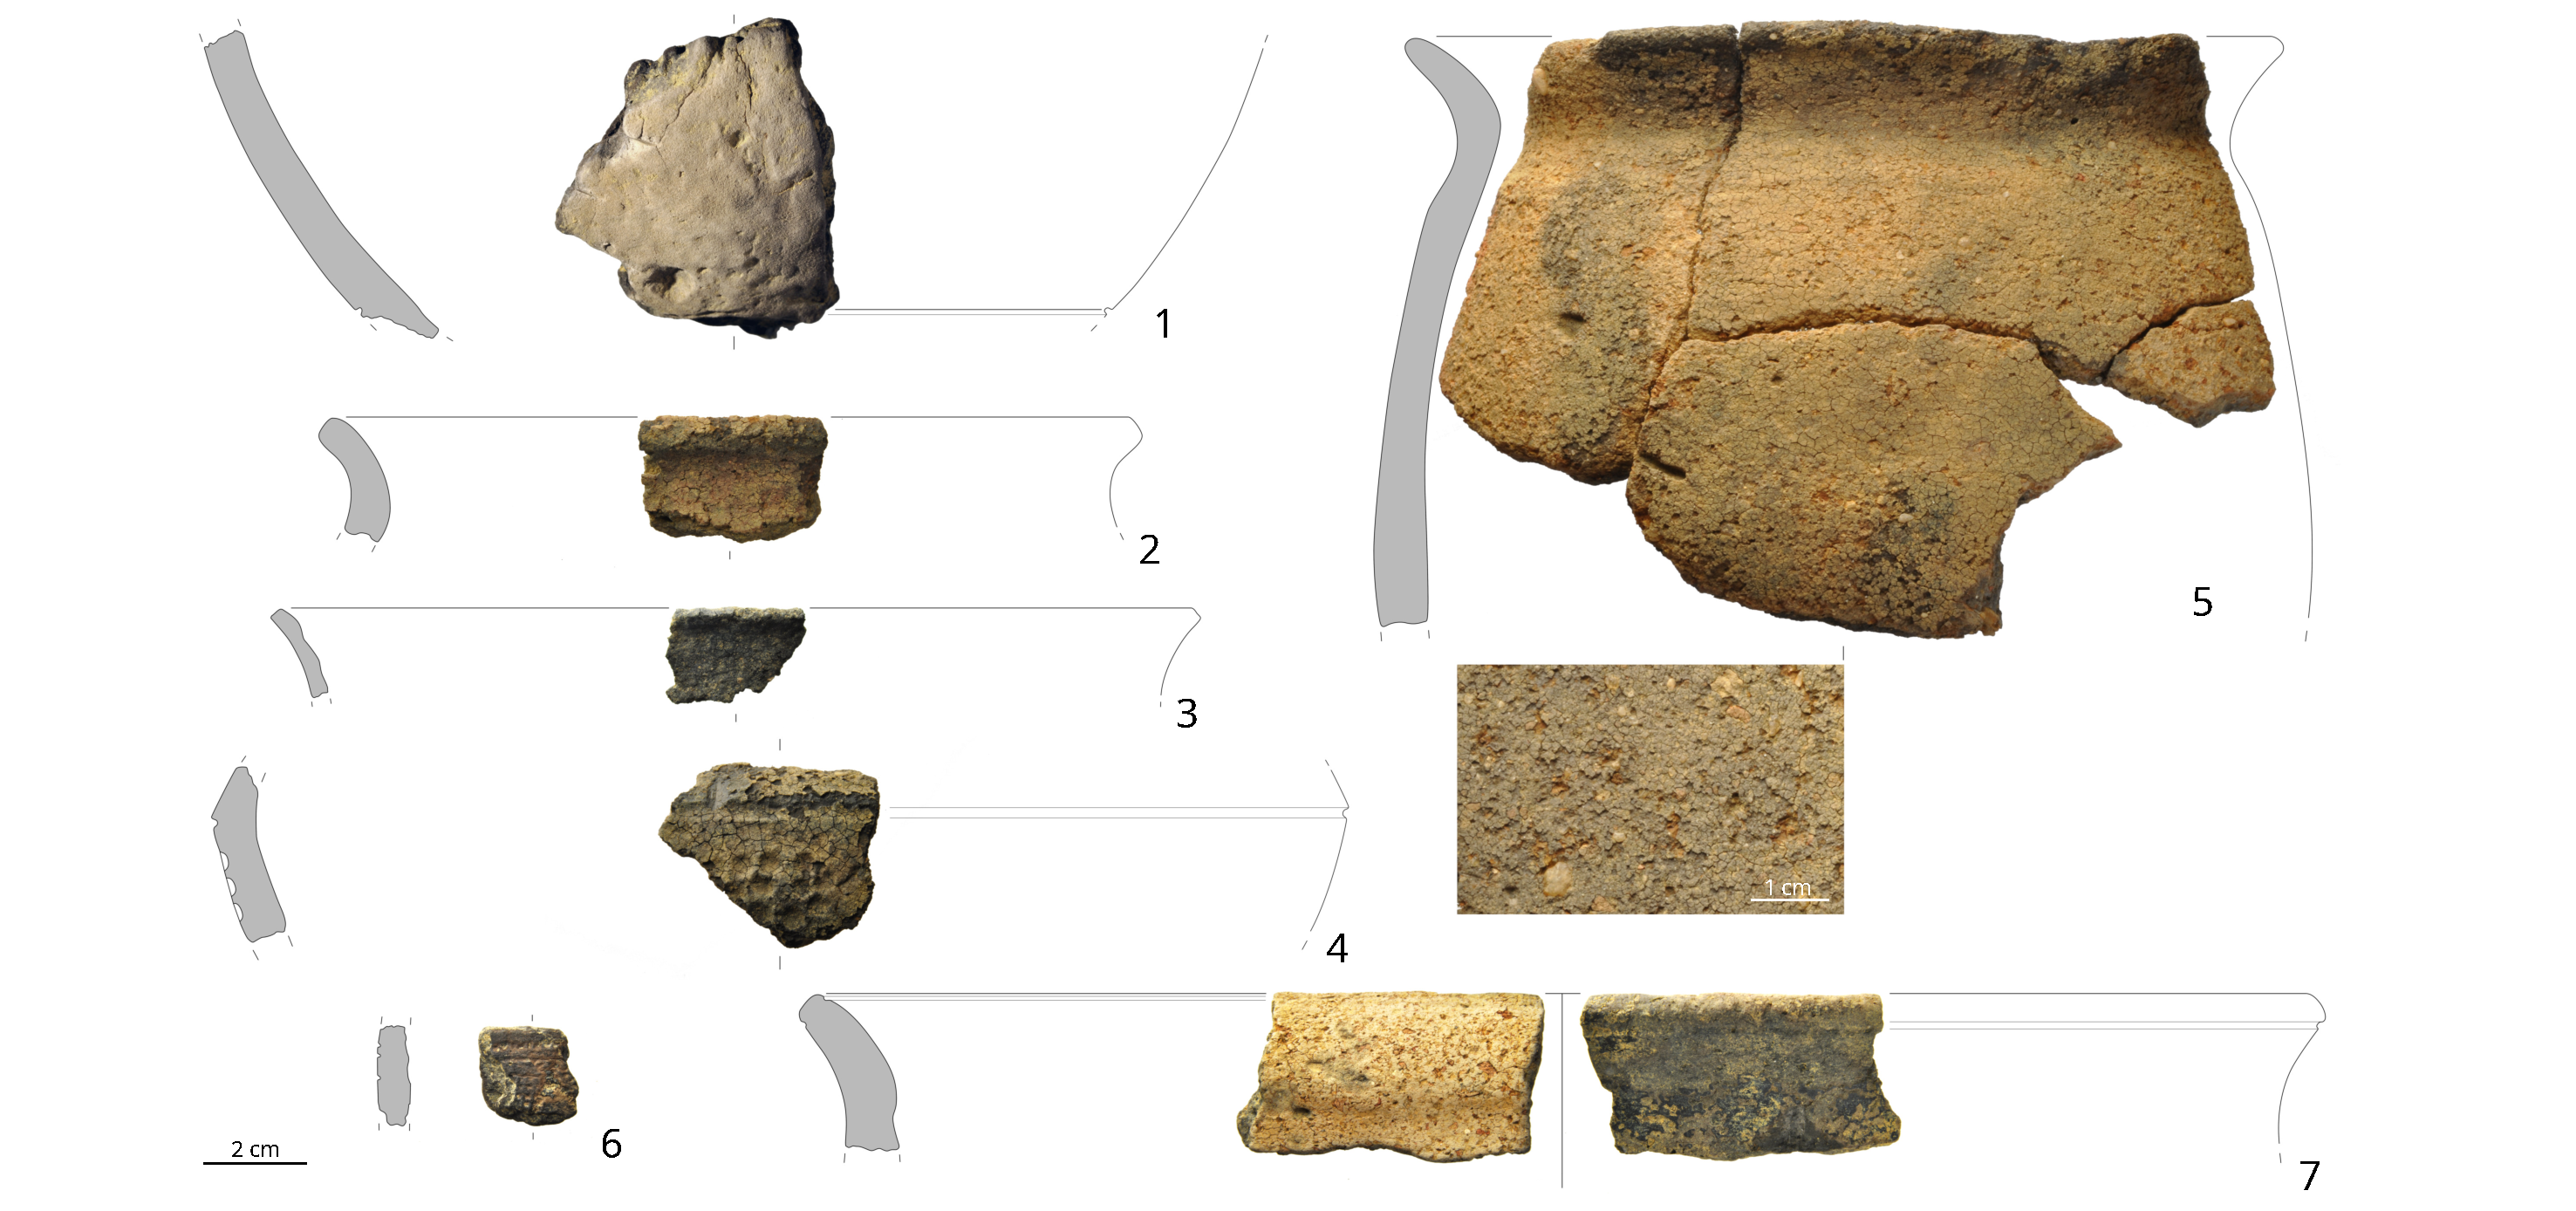
\includegraphics[width=\textwidth]{Fig_SNP-03_Pottery.pdf}
	% 1: SNP-01-7:1 #43
	% 2: 
	% 3: 
	% 4: 
	% 5: SNP-03-4:1 #42
	% 6: 
	% 7: SNP-03-7:1 #44
	% ---
	% SNP-03-4:4    #45
	% SNP-03-4:5    #46
	\caption{Diagnostic pottery uncovered within the Salonga national park.}
	\label{fig:snp.pottery}
\end{figure*}

\begin{table*}[p]
	\centering
	{\scriptsize \begin{tabular}{@{}lrrrrrrlrll@{}}
			\toprule
			\textbf{Loc} & \textbf{D} & \textbf{Obj} & \textbf{tsID} & \textbf{Wt} & \textbf{Qty} & \textbf{Size} & \textbf{Type} & \textbf{tW} & \textbf{Fabric} & \textbf{Notes}    \\
			\midrule
			SNG-01 & 60-70 & 1 & 43 & 55.9 & (8) & 70 & B & 8.5 & 1d & \begin{tabular}[c]{@{}l@{}}cf. Bokuma style; base with\\ groove (cf. Wotzka 1995: 400\\ Pl.6 B10)\end{tabular} \\
			SNG-03 & 10-20 &  &  & 11.8 & (2) & 70 & W & 9.5 & 8a &  \\
			SNG-03 & 10-20 &  &  & 4.2 & 2 & 30 & W &  & 4/5/8 &  \\
			SNG-03 & 30-40 &  &  & 1.5 &  & 30 & W & 5.5 & 1a & \begin{tabular}[c]{@{}l@{}}comb impressions; sponge\\ spicules under refelctive light\\microscope\end{tabular} \\
			SNG-03 & 30-40 &  &  & 2 &  & 30 & R & 5 & 4a & \begin{tabular}[c]{@{}l@{}}rim type B2 (cf. Seidensticker\\ 2021: 232 Fig. 8)\end{tabular} \\
			SNG-03 & 30-40 &  &  & 7.2 & 4 & 30 & W &  & 4/5/8 &  \\
			SNG-03 & 40-50 &  &  & 33.6 & 9 & 30 & W &  & 4/5/8 &  \\
			SNG-03 & 30-40 & 1 & 42 & 326,1 & (10) & 200 & R & 9 & 8a & \begin{tabular}[c]{@{}l@{}}vessel type B4 (cf. Seidensticker\\ 2021: 30 Fig. 5)\end{tabular} \\
			SNG-03 & 30-40 & 2 &  & 9.2 &  & 70 & R & 9.5 & 4b & \begin{tabular}[c]{@{}l@{}}rim type B2 (cf. Seidensticker\\ 2021: 232 Fig. 8)\end{tabular} \\
			SNG-03 & 30-40 & 3 &  & 12.4 &  & 70 & W & 8.5 & 4a & \begin{tabular}[c]{@{}l@{}}potential carinated bowl\\ with horizontal groove and\\circular impressions\end{tabular} \\
			SNG-03 & 30-40 & 4 & 45 & 5.3 &  & 70 & W & 9.5 & 4a &  \\
			SNG-03 & 30-40 & 5 & 46 & 7.8 &  & 70 & W & 7 & 4a &  \\
			SNG-03 & 30-40 & 6 &  & 2.3 &  & 70 & W & 5 & 1b & highly eroded \\
			SNG-03 & 30-40 &  &  & 63.3 & 7 & 70 & W &  & 4/5/8 &  \\
			SNG-03 & 30-40 &  &  & 58 & 20 & 30 & W &  & 4/5/8 &  \\
			SNG-03 & 50-60 &  &  & 3.5 & 2 & 30 & W &  & 4/5/8 &  \\
			SNG-03 & 60-70 & 1 & 44 & 22.9 &  & 70 & R & 10 & 8a & \begin{tabular}[c]{@{}l@{}}rim type B2 (cf. Seidensticker\\ 2021: 232 Fig. 8) and groove\\under the rim\end{tabular} \\
			SNG-03 & 60-70 & 2 &  & 8.3 &  & 70 & R & 6.5 & 4a & \begin{tabular}[c]{@{}l@{}}rim type B2 (cf. Seidensticker\\ 2021: 232 Fig. 8)\end{tabular} \\
			\bottomrule
	\end{tabular}}
	\caption{Pottery uncovered within the Salonga National Park. For the precice locations (Loc) see Fig.~\ref{fig:snp.map}. Depth (D) is recorded in centimeters below the surface. The corresponding identification number of the studied thin-sections (tsID) corresponds to the number in the label in Tab.\ref{tab:samples}. The weight (Wt) is recorded in gram. While the number of sherds (Qty) is given for a distinct unit of sherds with matching features from the same spit, vessel units combined from multiple sherds are listed in parentheses. The size was recorded following the system by \citet[89]{Clist.2004}. The type of sherd (Type) differentiates between fragments of the rim (R), wall (W) or base (B) of a vessel. The thickness of the wall (tW) was recorded in millimeter and rounded to a precision of 0.5~mm. The macroscopic fabrics (Fabric) was recorded following \citet[60--69 Tab.~11]{Seidensticker.2021e}.}
	\label{tab:snp.pottery}
\end{table*}

\section{Wafanya and Monkoto on the Luilaka river}

To contextualize the pottery found in the pedo-anthracological test pits, the inventories of the nearby sites Wafanya and Monkoto were sampled from the inventory of the \textit{River Reconnaissance Project}. In 1983, both sites were surveyed and excavations were conducted in Wafanya \citep[399--400]{Wotzka.1995}. Wafanya is located about 44~km downriver from the pedo-anthracological test pits, and Monkoto about 13~km upriver (Fig.~\ref{fig:map}). 51 sherds were found during surveys at Monkoto. The surveys of the modern village and missionary as well as nine out of 16 small test unites ("Bodeneinschläge") at Wanfanya yielded 166 sherds \citep[399--400]{Wotzka.1995}. Excavations were conducted at three locations following the test units: two smaller 1~\texttimes~1.5~m and one 2~\texttimes~2.9~m big trench \citep[360--368]{Wotzka.1995}. These trenches yielded another 522 sherds. The most elaborated stratigraphy, consisting of seven layers, was observed in the biggest trench (WAF~83/16). 

\begin{figure}[H]
	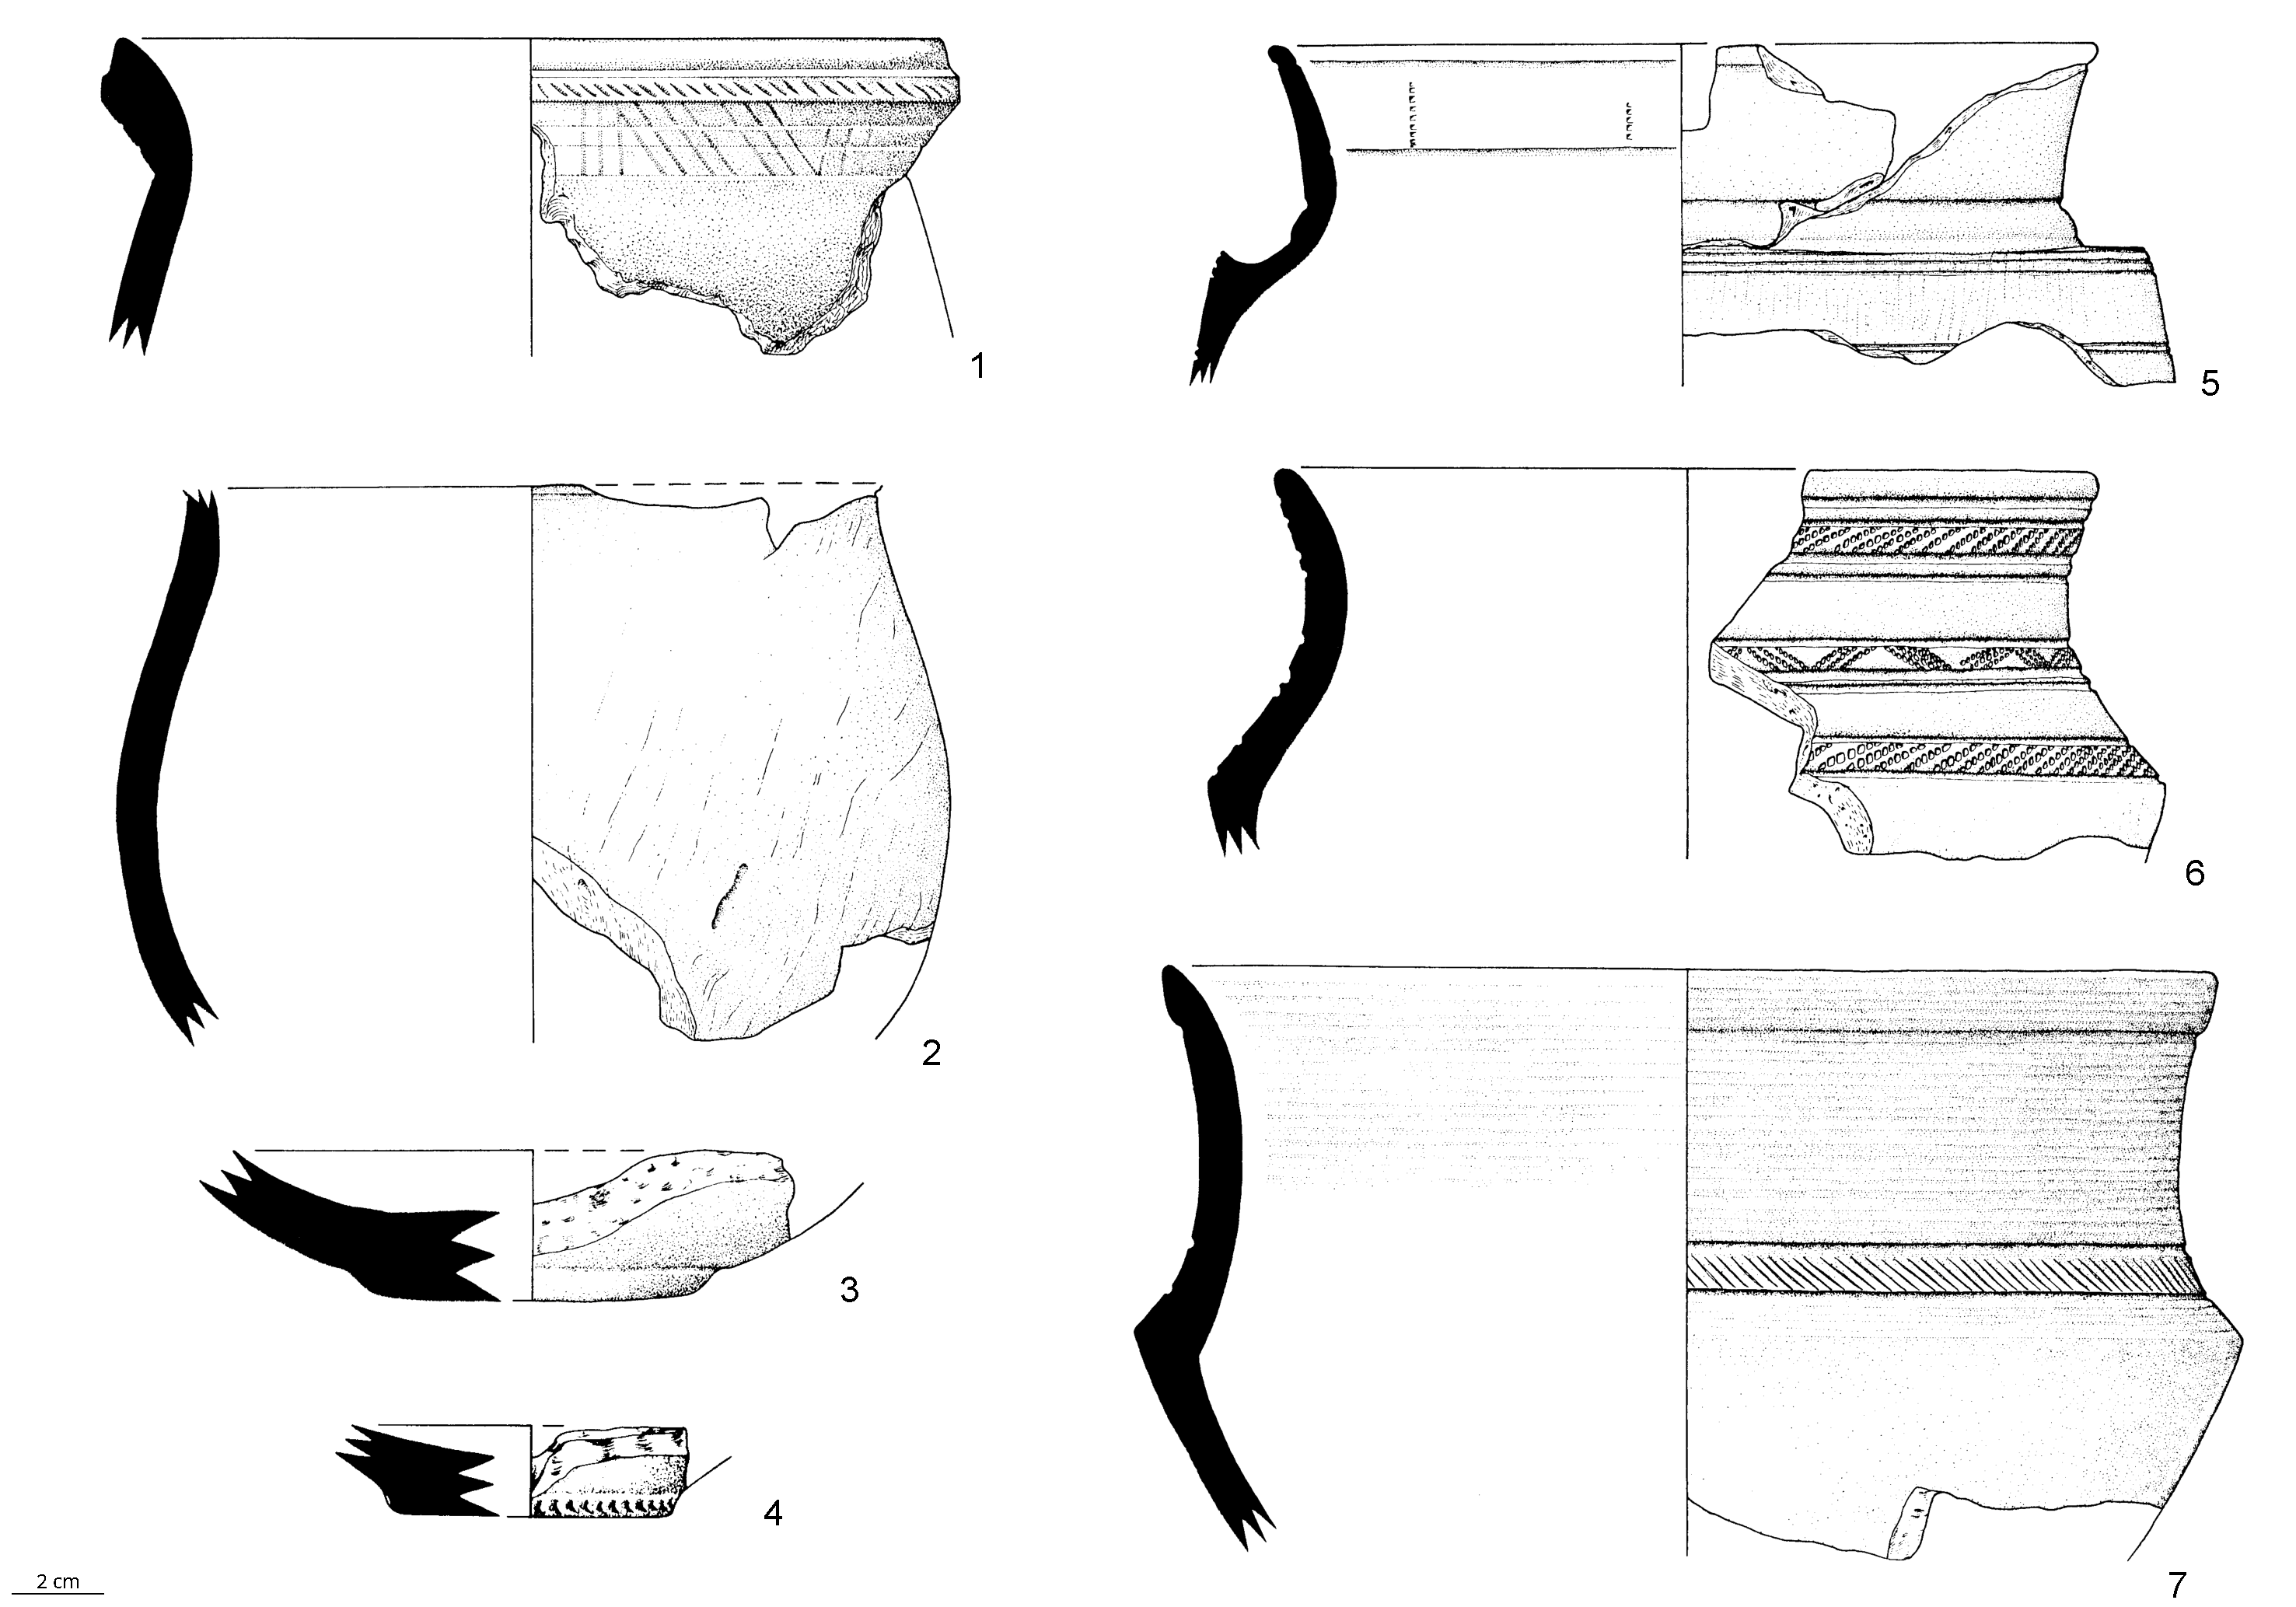
\includegraphics[width=\textwidth]{Fig_WafanyaMonkoto_PotterySampled.pdf}
	% 1: MON 83/101:1    #50 (72.5)
	% 2: WAF 83/16-2:1   #47 (70.10)
	% 3: MON 83/101:3    #51 (72.6)
	% 4: MON 83/101:4    #52 (71.6)
	% 5: WAF 83/16-5:33  #96 (96.5)
	% 6: WAF 83/16-2:3   #48 (69.6)
	% 7: WAF 83/16-7-1:2 #49 (69.9)
	\caption{Sampled pottery from Wafanya \citep[2,5--6;][503 Pl.~69--504 Pl.~70]{Wotzka.1995} and Monkoto (1,3--4) representing the pottery styles Monkoto (1--3), Bekongo (5--6) and Longa (7) }
	\label{fig:wafmon.pottery}
\end{figure}

The local sequence of pottery styles at Wafanya is comprised of ten styles (Fig.~\ref{fig:chrono}.B). Wafanya is the southern- and eastern-most site yielding Imbonga style pottery, the earliest known pottery style in the Inner Congo Basin dating to between the 4th and 2nd century BCE \citep[59--68, 544--545 map 2]{Wotzka.1995}. A single sherd of this style was found between the Luilaka river and the missionary \citep[WAF~83/105;][399, 505 Pl.~71.1]{Wotzka.1995}. The bulk of the ceramics found at Wafanya (55~\%) is part of the style group with the same name dating into the 12th to 13th century CE \citep[163--167]{Wotzka.1995}, followed by pottery of the Longa style dating into the 11th to 14th century CE \citep[23~\%;][121--128]{Wotzka.1995} (23~\%). The surveys at Monkoto yielded 44 sherds, with 75~\% being part of the pottery style with the same name dating into the 1st century BCE to 2nd century CE \citep[94--100,400]{Wotzka.1995}.

\bibliographystyle{elsarticle-harv}
\bibliography{bib.bib}

\end{document}
